%%%%%%%%%%%%%%%%%%%%%%%%%%%%%%%%%%%%%%%%%%%%%%%%%%%%%%%%%%%%%%%%%%
% Capitoli già visti a lezione								    %
%%%%%%%%%%%%%%%%%%%%%%%%%%%%%%%%%%%%%%%%%%%%%%%%%%%%%%%%%%%%%%%%%%
\newpage
\section{Acciai inossidabili austenitici}
\subsection{Tattamenti termici applicabili}
Durante un'eventuale saldatura, il processo di raffreddamento non è 
controllato per cui non si è sicuri se il processo di stabilizzazione sia 
ancora valido. Perciò è meglio optare per degli acciai low carbon.
Per gli acciai austenitici la sensibilizzazione avviene ad una certa distanza 
dal cordone di saldatura. Per quelli feritici invece si avvicina al cordone
per via delle caratteristiche dell'acciaio.

\subsubsection{Trattamento di distensione}
Si riscalda l'acciaio ad una temperatura inferiore alla temperatura di inizio
sensibilizzazione. Tenendo il processo per circa $30min \div 2h$.
Successivo raffreddamento in aria calma. 
Si fa per eliminare le tensioni interne generate per qualsiasi motivo.
Ciò riduce il pericolo della \emph{tensocorrosione}.
Il processo si esegue solo in caso in cui si presume che ci sia tale moti vo di corrosione.

Gli acciai inox austenitici non hanno particolari caratteristiche meccaniche 
Risultano però molto deformabili e hanno una buona capacità di incrudimento.
È possibile che si vada a generare l'effetto \ac{TRIP} (visto in precedenza).
Per via del fatto che essendo deformato a freddo, c'è la tendenza che 
l'austenite venga trasformata in martensite (Sotto la temperatura $M_d$ 
ovvero quella temperatura che permette la trasformazione di austenite in
martensite a fronte di una deformazione).

\begin{figure}
\centering
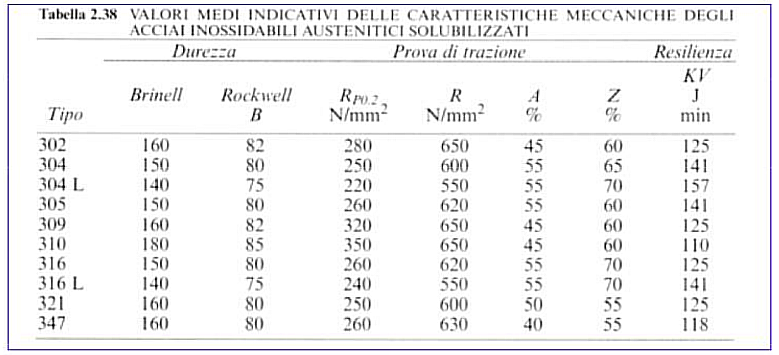
\includegraphics[width = \textwidth]{CaratMeccInoxAust}
\caption{Caratteristiche meccaniche degli acciai inossidabili austenitici dopo trattamento di distensione}
\label{fig:CaratMeccInoxAust}
\end{figure}

Gli acciai austenitici hanno una buona resistenza al Creep ovvero
uno sforzo ad alta temperatura a carico costante.

Riassumendo:\\
Gli acciai inossidabili austenitici hanno un buon comportamento a bassa 
temperatura in quanto non presentano la transizione duttile-
fragile. Ad alta temperatura bisogna stare attenti alle temperature  
critiche di sensibilizzazione.
Possono resistere bene alla corrosione in ambienti aggressivi.
Sono molto utilizzati in quei campi dove la sicurezza è di 
fondamentale importanza.

I super-austenitici vengono chiamati così perché hanno valori di $PREN>40$.


\section{Acciai inossidabili ferritici}
Sono ancora acciai monofasici. Secondo l'\ac{AISI} sono 
designati come 4XX. Non è completamente indicativa della struttura in
quanto ci sono sia i ferritici che i martensitici con la stessa nomenclatura.

La tipica lega dei ferritici prevede leghe: Fe-C-Cr.
Dunque si scelgono questi acciai quando si vuole optare per una scelta più 
economica.
Hanno struttura ferritica a tutte le temperature. Fanno eccezione gli acciai
detti \emph{semiferritici} che se scaldati e portati in austenitizzazione 
e raffreddati velocemente formano della martensite.
In genere non sono adatti ai trattamenti termici. E sottoporli a tali 
trattamenti compromette la resistenza a corrosione.
Sono suscettibili al rinforzo per incrudimento, comunque meno di quanto fanno 
gli austenitici.
Un acciaio ferritico di riferimento è l'\texttt{\ac{AISI} 430}.
\missingfigure{Aggiungere Metallografia AISI 442}

\todo[inline]{Vedi la tabella della comparazione delle proprietà}

Possibile formazione della fase $\sigma$ che contiene molto cromo 
andando ad infragilire la struttura e sensibilizza alla corrosione 
intergranulare.

\subsection{Trattamenti termici}
Non si vanno a migliorare le caratteristiche meccaniche come per gli 
asutenitici. Piuttosto vengono tamponate delle situazioni in cui gli 
acciai potrebbero essere più sensibili.

\subsubsection{Ricottura di ricristallizzazione}
Si effettua per ricristallizzare un materiale che precedentemente ha subito 
una deformazione plastica.
Non si deve mai superare la temperatura critica dei $850\unit{\celsius}$ per 
cui il grano ferritico tenderebbe a ingrossare troppo.
Siccome stiamo effettuando una ricristallizzazione non è detto che si possa 
effettuare una successiva deformazione (soprattutto se il pezzo è già 
stato formato).
Si preferisce abbondare col raffreddamento, di solito fatto in acqua.
Perché si può incorrere in fenomeni di infragilimento.
\begin{description}
\item[Infragilimento a $457\unit{\celsius}$] Si ha una decomposizione della 
fase $\alpha$. Da lì inizia a formarsi, per via dell'alta percentuale di 
cromo, da cui si forma sia fase $\alpha$ che $\alpha'$.
Dove la prima è molto ricca di Fe, l'altra più ricca di Cr.
Se ne moficano le caratteristiche meccaniche e aumenta la TTDF%
\todo{acronimo}.
È un problema reversibile, si può scaldare nuovamente il materiale per 
poi raffreddarlo più velocemente.
\item[Infragilimento per fase $\sigma$] È reversibile, in maniera simile 
a quanto visto prima. Bisogna stare attenti alla temperatura di 
riscaldamento che deve essere $\approx 800\unit{\celsius}$. 
\end{description}

Ciò pone questi acciai in situazioni di sensibilizzazione
che può verificarsi a $T > 950\unit{\celsius}$. Perciò bisogna porre 
particolare attenzione alle saldature.

La motivazione è ancora in fase di studio. Perciò non è completamente chiara.
\missingfigure{Aggiungere i grafici della sensibilizzazione}
Si potizza che: a causa della non omogeneità della matrice del materiale, si 
vadano a formare delle isole austenitiche interne al grano ferritico.
Allora possono formarsi dei carburi di ferro che precipitano, risultando più 
sensibili alla corrosione.
Non esiste un processo di stabilizzazione del materiale, perché il processo
di sensibilizzazione non è strettamente legato alla precipitazione di 
carburi di cromo. Perciò non è così efficace.

\subsubsection{Acciai ferritici ELI}
Si tratta di leghe Fe-Cr-Mo a bassisimi tenori di C e N.
Presentano alta resistenza alla tensocorrosione.

\section{Acciai inossidabili Martensitici}
Si applicano per quelle applicazioni in cui si vuole una buona resistenza
alla corrosione (ben maggiore dei CORTEN) ma non si vuole rinunciare
alle caratteristiche meccaniche.
\todo{Aggiungere i tenori di carbonio}
Sono scuscettibili ai trattamenti termici di indurimento in quanto presentano 
i punti critici $A_1$ e $A_3$. 
Dopo la tempra presentano una struttura martensitica o martensitica con 
carburi. Per cui si raggiungono durezze molto elevate $\approx 45\unit{HRC}
\div 65\unit{HRC}$.

Non sono facili da saldare in quanto i tenori di carbonio sono parecchio 
elevati.

Una designazione tipica di riferimento è l'\texttt{AISI 410}.

\subsection{Trattamenti termici}
\todo[inline]{vedi slides per magiore completezza}

Hanno elevata temprabilità e vengono in genere temprati in olio e in aria, 
detti anche autotempranti (la scelta dipende dagli spessori).

\section{Acciai inossidabili PH}

Acciai non più monofasici, andando ad interrogare gli acciai duplex.
\ac{PH}. 
Sono stati sviluppati per richieste dell'industria aeronautica e bellica.
Hanno elevate caratteristiche meccaniche al contempo elevate caratteristiche
alla corrosione.
Tali caratteristiche si sono ottenute grazie al processo di indurimento per
precipitazione.
Spesso vengono nominati tramite il nome commerciale piuttosto della
designazione normativa.
Secondo l'\ac{AISI} sono la serie 6XX. Come riferimento al
\texttt{AISI 630}.

\todo{\\Aggiungere eventuali nomenclature europee}
Si nota, dalla nomenclatura europea, che i tenori di carbonio è molto
molto basso $0.01\%$ per alcune formulazioni.
Questa caratteristica non è troppo distante dagli acciai austenitici.
Ciò impone che le caratteristiche meccaniche vengano demandate ai (molti)
elementi in lega tipo Cu, Ti, Al. Si demanda alla precipitazione di altre 
soluzioni.
Ad esempio spesso si hanno precipitazioni tipo: $Ni_3X$ dove $X$ è un
altro elemento in lega.
Si può avere la presenza di precipitati di carburi o nitrocarburi. In modo da formulare precipitazioni fini e disperse si possono incrementare la resistenza meccanica dell'acciaio come già visto anche per gli \ac{HSLA}.

Vengono suddivisi in tre classi:
\begin{description}
\item[Martensitici] come riferimento si prende il \texttt{17-4 PH} che corrisponde al \texttt{AISI 630}. Tra l'altro è l'acciaio più diffuso per questa tiplogia di acciai
\item[Semi-austenitici] come riferimento si può considerare il \texttt{17-7 PH} che equivale all'\texttt{AISI 631}. Vengono forniti allo stato austenitico. Dopo tutto il processo di produzione e trattamento termico finale si ha una matrice non più austenitica ma martensitica. Da qui il nome semi-austenitico.
\item[Austenitici] Hanno più alto contenuto di P, per cui viene evidenziato nella sigla omettendo la H: \texttt{17-10 P} mentre non ha una corrispondenza perfetta nella nomenclatura \ac{AISI}.
\end{description}
La nomenclatura indica nelle prime cifre la percentuale del tenore di Cr, nelle seconde la percentuale di Ni.
Tra l'altro il tenore di Ni abbassa i punti $M_s$ e $M_f$ si abbassano per cui si favorisce una matrice austenitica piuttosto di quella martensitica.
Inoltre grazie alla presenza in lega di particolari elementi si sfrutta un'indurimento misto tra precipitazione di carburi (anche se il carbonio è molto poco) e altre precipitazioni.
Si ricorda che affinché sia efficace la precipitazione, i precipitati devono essere piccoli e dispersi. Altrimenti si infragilisce la struttura peggiorando la situazione.
\missingfigure[figcolor = white]{Aggiungere tabella per gli acciai PH} 

\subsection{Trattamenti termici}
Per gli acciai \ac{PH} subiscono un trattamento termico che è comune anche agli acciai
\begin{itemize}
\item acciai Maraging, acciai martensitici induriti tramite precipitazione.
\item leghe di alluminio
\item Superleghe
\end{itemize}
\missingfigure{Grafico trattamento termico PH}

Il processo è il seguente
\begin{enumerate}
\item Solubilizzazione tra i $750\div1050\unit{\celsius}$
\item Tempra
\item Invecchiamento.
\end{enumerate}
Si ottiene un'indurimento per precipitazione dovuto a precipitazione della matrice di composti intermetallici, carburi, nitruri o fasi contenenti Cu o altri elementi.

Ora vediamo come cambia il processo di produzione per le varie classi di \ac{PH}.

\subsection{Acciai PH Martensitici}
Sono i più impiegati e vengono forniti già allo stato martensitico.
Contengono una buona dose di Cu $\approx 4\%$ e spesso presentano anche del Nb per realizzare dei carburi di niobio.
$M_f$ è maggiore della temperatura ambiente dunque si ha una matrice martensitica dopo rapido raffreddamento.

Combinano elevata resistenza meccanica e buona resistenza alla corrosione.
Hanno un costo decisamente elevati.
Le applicazioni sono molteplici grazie alla loro diffusione: sono stati sviluppati per l'ambito militare e aerospaziale. Ora si trovano in componentistica per automobili, ingranaggi e sensoristica. Vengono sfruttati anche per la manifattura additiva.

Il trattamento termico non è molto diverso da quello visto in precedenza.
\missingfigure{Grafico ciclo termico PH Martensitici}
Si realizza una solubilizzazione a $1050\unit{\celsius}$ e tempra. presentano una martensite duttile per il basso tenore di carbonio $\approx 0.05 \div 0.07\%$.
Dopo l'invecchiamento con $T = 480 \div 620\unit{\celsius}$. La matrice risulta rinforzata da precipitati nanometrici, anche di tipo $Ni_2X$ e fasi CFC ricche di Cu nel caso del \texttt{17-4 PH}
\missingtable{Tabella caratteristiche meccaniche}

\subsection{Acciai PH Austenitici}
Bisogna ricordare che in questo caso $M_s$ e $M_f$ sono sotto la temperatura ambiente (di molto). Per cui non si ha formazione di martensite.
\missingfigure{Ciclo termico PH aust.}
A temperatura ambiente post tempra, vengono effettuate le lavorazione a freddo per guadagnare resistenza meccanica e poi effettuare l'invecchiamento.
Resta una buona riserva plastica anche dopo l'invecchiamento per via della struttura austenitica.
\missingtable{Tabella valori caratteristiche meccaniche}

\subsection{Acciai PH Semi-Austenitici}
$M_f$ è sotto temperatura ambiente, perciò sarà necessario un rappreddamento sotto temperatura ambiente.
Per favorire il passaggio da austenite a martensite (Passaggio di condizionamento) per trasformare l'austenite in martensite.
Grazie a questo processo si riesce ad alzare $M_s$ e $M_f$.
\todo{\\Vedi descrizione ciclo termico nelle slide}
\missingfigure{Ciclo termico PH semi-aust.}

\missingtable{Valori caratteristiche meccaniche PH Semi-Aust.}

\subsection{Considerazioni conclusive}
Con questi acciai si riescono a raggiungere delle ottime caratteristiche meccaniche, anche superiori agli inossidabili martensitici; ottenendo delle resistenze alla corrosione confrontabili con gli inossidabili austenitici.

Presentano una buona saldabilità! ad eccezione per gli acciai P, perché il fosforo tende a generare fasi basso-fondenti, rischiando di generare delle cricche a caldo.

Il trattamento di invecchiamento non provoca distorsioni quindi si hanno dei costi maggiori degli inossidabili. Viene compensato dai più ampi limiti d'impiego dell'acciaio.


\section{Acciai Inossidabili Duplex}
Da non confondere con gli acciai \ac{DP} che presentano una combinazione tra ferrite e martensite (più eventuale bainite residua).
In questo caso si parla di acciai che propongono metà struttura austenitica e metà in fase ferritica.

Tale composizione è ottenuta tramite il bilanciamento della lega Cr-Ni-Mo.

Sono acciai con costo medio-alto. Vengono impiegati in ambienti in cui
\todo{\\Vedi la slide per gli impieghi.}

\missingfigure{Composizione struttura.}

Vengono sfruttati per l'ambiente chimico-petrolchimico e strutture \eng{off-shore}.
Sono saldabili e presentano una buona resistenza meccanica e alla corrosione. Non presentano ossidazione ad alta temperatura.
Possono essere suscettibili all'infragilimento a $475\unit{\celsius}$.

\missingfigure{Inserire tabelle nomenclature acciai duplex}

Il prefisso "super" indica un valore di \ac{PREN} > 40\%.
Indice che questi materiali sono particolarmente resistenti ad attacchi corrosivi.
\begin{equation}
PRE_N = \%Cr + 3.3 \%Mo + 30 \%Ni
\end{equation}
\todo{\\Verificare le formule del PREN}

\missingfigure{Metallografie fenomeno pitting}

Il \eng{pitting} tende a formarsi sulla ferrite che non sull'austenite.

\subsection{Trattamento termico per i duplex}
Dal diagramma in figura, si può stimare quanta parte di fase $\delta$ e $\gamma$. La frazione delle due dipende dagli elementi in lega e dalla temperatura di raffreddamento.
Di solito gli acciai duplex vengono \textbf{solubilizzati} tra i $1000\div 1100\unit{\celsius}$. Viene seguito da una raffreddamento rapido per bloccare l'evoluzione delle due fasi. In più si vogliono evitare i fenomeni di infragilimneto e sensibilizzazione del materiale.

\missingfigure{Grafico curve di Bhain}

Attenzione al \ac{PREN}: quello è un indice sulla base della composizione chimica del materiale. Se la microstruttura ha generato delle fasi infragilenti o sensibilizzanti, sicuramente il comportamento del materiale non è quello dato dalla sola composizione chimica. 